\graphicspath{{images/}}

\section*{Turingmaschinen}

\begin{theorem}{Turingmaschine (TM)} $M=\left(Q, \Sigma, \Gamma, \delta, q_{0}, \sqcup , F\right)$

    \begin{minipage}{0.45\linewidth}
        $Q$: Menge von Zuständen

        $\Sigma$: Alphabet der Eingabe

        $\Gamma$ und $\Sigma \subset \Gamma$: Bandalphabet
    \end{minipage}
    \begin{minipage}{0.55\linewidth}
        $q_{0} \in Q$: Anfangszustand

        $F \subseteq Q$: Akzeptierende Zustände

        ${ }_{\sqcup }$: Leerzeichen mit ${ }_{\mu} \in \Gamma$ und ${ }_{\mu} \notin \Sigma$
    \end{minipage}

    Übergangsfunktion: $\boldsymbol{\delta}: \boldsymbol{Q} \times \boldsymbol{\Gamma} \rightarrow \boldsymbol{Q} \times \boldsymbol{\Gamma} \times \boldsymbol{D}, \boldsymbol{D}=\{\boldsymbol{L}, \boldsymbol{R}\}$
    
    \vspace{1mm}

    Sie bestehen aus einem Lese-/Schreibkopf und einem unendlichen Band von Zellen.

    \vspace{1mm}

    Sie bildet das 2-Tupel $(q, X)$ auf das Tripel $(p, Y, D)$

    \begin{minipage}{0.45\linewidth}
        $D=$ Direction

        $X=$ Read

        $Y=$ Overwrite
    \end{minipage}
    \begin{minipage}{0.5\linewidth}
       $q, p \in Q$ und $X, Y \in \Gamma$

       \emph{$q-X / Y, D \rightarrow p$}
    \end{minipage}

\end{theorem}

\begin{definition}{Band} Unterteilt in Zellen mit jeweils einem beliebigen Symbol
    
    Beinhaltet zu Beginn die Eingabe, d.h. ein endliches Wort aus $\Sigma^{*}$. Alle anderen Zellen enthalten das besondere Symbol $\sqcup$
\end{definition}

\begin{definition}{Konfiguration}einer TM $M$ wird eindeutig spezifiziert durch:

    Zustand der Zustandssteuerung, Position des Lese-/Schreibkopfes und Bandinhalt
\end{definition}

\begin{concept}{Arten von TMs} $\forall$ Sprachen L gleich akzeptierend wie normale TM

    \vspace{1mm}

    \begin{minipage}{0.45\linewidth}
        \begin{itemize}
            \item semi-unendliches Band
            \item mit Speicher
            \item mit Zählern
        \end{itemize}
    \end{minipage}
    \begin{minipage}{0.45\linewidth}
        \begin{itemize}
            \item mehrere Stacks
            \item mehrere Spuren
            \item mehrere Bändern
        \end{itemize}
    \end{minipage}
\end{concept}

\begin{example2}{Mehrband-Maschine}\\
    Spezifizieren Sie eine TM $M_{4}$, welche die Subtraktion von zwei natürlichen Zahlen $(a-b$, mit $a \geq b)$ realisiert.\\
    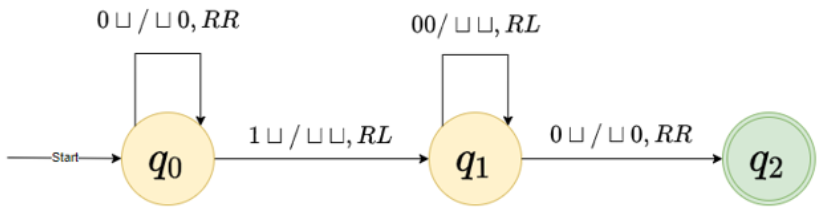
\includegraphics[width=0.5\linewidth]{mehrband_maschine1.png}\\
    Beispiel: $4-2=2$\\
    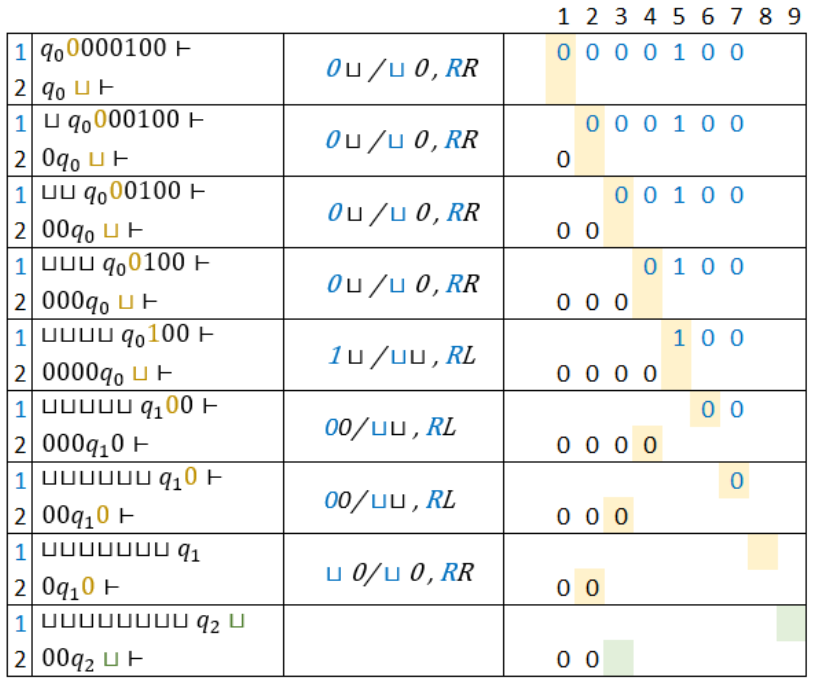
\includegraphics[width=1\linewidth]{mehrband_maschine2.png}
\end{example2}

